\documentclass{journal}
\usepackage{graphics,graphicx}
\usepackage{hyperref}
\usepackage{fullpage}
\usepackage{pdflscape}
\usepackage{tikz}
\usepackage{gantt}
\usepackage{setspace}
\usepackage{enumitem}

\onehalfspacing

\begin{document}

\bibliographystyle{IEEE}
\nocite{*}
\title{Interactive Graduate Student Information Database}
\subtitle{Midterm Report} 
\author{Kartik Thakore (250313003)\\kthakore@uwo.ca}
\maketitle

\begin{abstract}
The purpose of this report is to document preliminary elicited requirements for the Interactive Graduate Student Information System (SIMS). Additionally, in accordance with the Agile project management methodology, a walk through of the first iteration is documented. Our first iteration includes two system critical features which will be used for iterative system development of the system. Database schemas and operational logic for user authentication and calculations for graduate student funding were accomplished.  A database schematic was designed after performing extensive analysis based on our specifications, data flow requirements and approved system critical assumptions. Data normalization was performed and a Representational State Transfer (REST) framework was implemented to combine components. Furthermore, unit and integration testing were performed with the preliminary implementation in place. For preparation of future iterations, a sign-off from end users and client is required. However, we have started the rapid prototyping of the e-signature component for the advisory meeting tracking feature. 
\end{abstract}



\section{System Overview}

The SIMS core is a secure application that aims to be flexible to handle business rules of varying graduate student programs. In the scope of this project however, focus will be placed on the Graduate Student Program at the BioMedical Physics program at University of Western Ontario. At the very least SIMS will hold graduate student, funding and advisory meeting data. Additionally SIMS will allow the program administrator to organize collected data into reports and to send automatic request for data to students. Also advisors and other faculty users will be able to see student data, progress and any advisory meetings they have attended. SIMS will also place an emphasis on providing security of student personal data and faculty identifications. Overall SIMS, will be replacing the current manual system of tracking students and their progress through graduate programs.

\subsection{Scope}

Figure \ref{fig:sysOver} shows the overview of the required system. The user will access the system via the Client and Tablet devices. The data from the tablet will be processed in the client and sent via the TCP/IP protocol to the Application Server (AppServer). The responsibility of the AppServer is to provide secure access, and host the application. The AppServer will communicate with the Services Server to add triggers and use the database. The AppServer and the ServicesServer will be located on a local network which is accessed via a Virtual Private Network (VPN).


Figure \ref{fig:Users} models the users of the SIMS system. The user groups can be broken down into 3 categories, the Student, the Faculty and the Technical Administrator. The technical administrator will have access only to the authentication data. While the student and the faculty will have access only to the tracked data. Additionally the faculty will have more access over the student. The role and operations requirements will be covered more in-depth in the system features.

\begin{figure}[!h]
\begin{center}
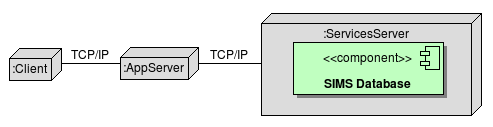
\includegraphics[width=522px]{diagrams/scope} \caption{ The proposed system } \label{fig:sysOver}

\end{center}
\end{figure}


\begin{figure}[!h]
\begin{center}
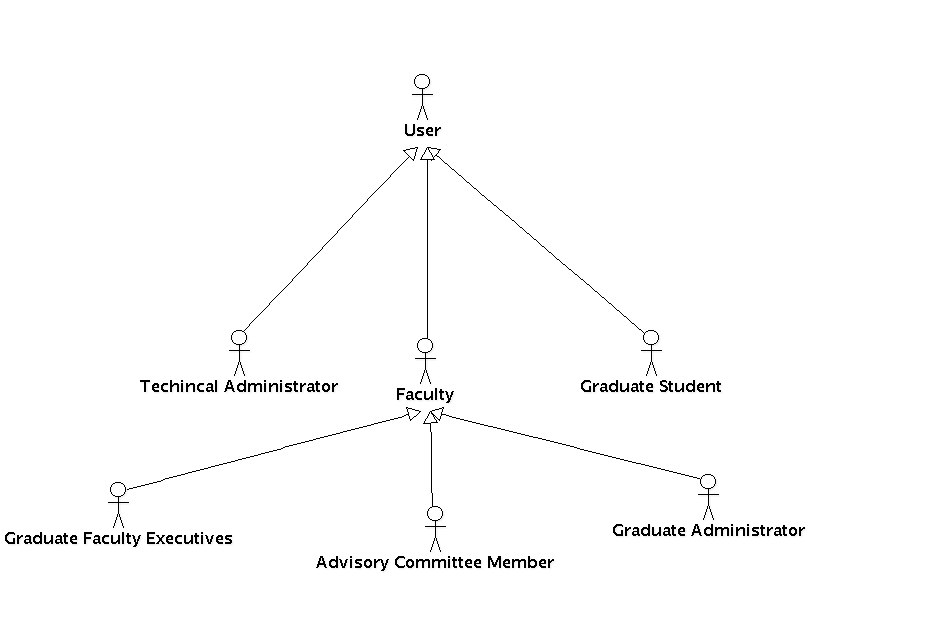
\includegraphics[width=468px]{diagrams/use_cases/UserHeirachy_uc} \caption{ Users of the SIMS system } \label{fig:Users}

\end{center}
\end{figure}



\subsection{Technical Environment}

SIMS will be built on the Linux Server platform for the Database and Application Server. The client will be limited to a Linux Operating System with the Firefox 3.6 web browser.  

\section{Specific requirements}
\subsection{External interface requirements}
\subsubsection{ Graphical User Interface }
The web interface is primary link for providing users with system functionality access. The web interface will require a specific web browser to be used in order to prevent any compatibility issues. 

\subsubsection{ Electrical Device Interface }
A hardware interface capable of recording electronic signatures from various stakeholders to create a e-record of the forms for added accessibility. The image captured by the signature pad will go through layers of encryption and image processing algorithms to be encrypted and then saved using an appropriate protocol in the database.


\subsection{System features}
\subsubsection{User Administration}

\begin{figure}[!h]
\begin{center}
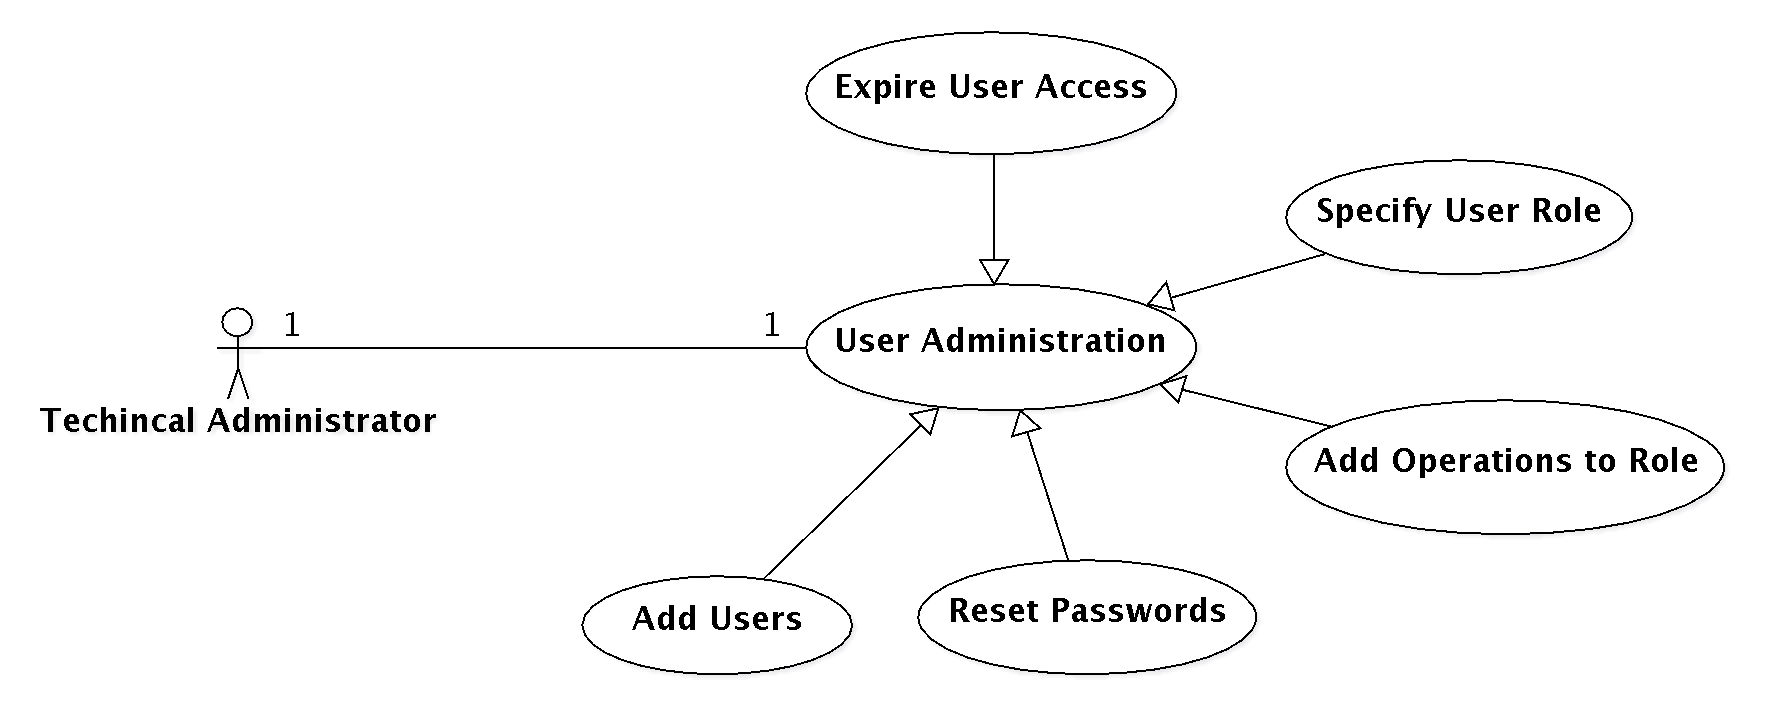
\includegraphics[width=440px]{diagrams/use_cases/TechAdmin_uc.png} \caption{ User Administration } \label{fig:UsersAdmin}

\end{center}
\end{figure}




\subsubsection{Personal Graduate Information}
\begin{enumerate}
\item Purpose:
\item Response sequence:
\item Associated Functional Requirements:
\end{enumerate}

\subsubsection{Program Information}
\begin{enumerate}
\item Purpose:
\item Response sequence:
\item Associated Functional Requirements:
\end{enumerate}


\subsubsection{Tracking Student Funding}
\begin{enumerate}
\item Purpose:
\item Response sequence:
\item Associated Functional Requirements:
\end{enumerate}


\subsubsection{Tracking Advisory Committee Meetings}
\begin{enumerate}
\item Purpose:
\item Response sequence:
\item Associated Functional Requirements:
\end{enumerate}


\subsubsection{Reporting Data}
\begin{enumerate}
\item Purpose:
\item Response sequence:
\item Associated Functional Requirements:
\end{enumerate}
\subsubsection{Email Triggering}
\begin{enumerate}
\item Purpose:
\item Response sequence:
\item Associated Functional Requirements:
\end{enumerate}

\subsubsection{Graphical User Interface}
\begin{enumerate}
\item Purpose: Provide an intuitive dossier format interface for users to see the student profile in a centralized location.
\item Response sequence: In order to access the GUI, the user will be required to login and will be taken to a dashboard which will have options to generate reports and search a student by their assigned id. Once selected the user will be able to see a student profile and be able to perform various functions based on their authentication scope as defined in the access control list.
\item Associated Functional Requirements:
\begin{enumerate}
\item Drill down: Functional Requirement 1
\begin{enumerate}
\item Sections: each student will have multiple sections that can be disabled or enabled.
\item Expansion: sections will expand to show summary of addition information.
\item Link: sections will link to sections pages for more detailed information.
\end{enumerate}
\end{enumerate}
\end{enumerate}
\subsubsection{Term Calculations}
\begin{enumerate}
\item Purpose: Calculate dates and event times for graduate student programs 
\item Response sequence: When a student profile and program is created the system will make triggers for relevant events to each milestone.
\item Associated Functional Requirements:
\begin{enumerate}
\item Milestones: Functional Requirement 1
\begin{enumerate}
\item Calculate start - end  Semester dates for Graduate Students
\item Calculate due dates and triggers for milestones
\end{enumerate}
\item Funding Calculations: Functional Requirement 2
\begin{enumerate}
\item Track funding availability for each semester and the source of funding
\item Show next date for major funding applications
\end{enumerate}
\end{enumerate}
\end{enumerate}
\subsubsection{Tracking}
\begin{enumerate}
\item Purpose: Track Major Milestones (grants, publications, exams etc) for graduate students through the program.
\item Response sequence: Data is updated according to business rules and workflow of the program and the student's progress.
\item Associated Functional Requirements:
\begin{enumerate}
\item Publications and Grants: Functional Requirement 1
\begin{enumerate}
\item Track student publications that have been published 
\item Track grants that have been received by the student
\end{enumerate}
\item Advisory Committee Members: Functional Requirement 2
\begin{enumerate}
\item Send trigger to student to form an Advisory Committee
\item Allow students, and advisory committees to store and track comments and discussions
\item Show calendar view of all meetings and results of the meetings
\item Allow for single or joint supervisors 
\item Track electronic submissions of advisory meeting form
\end{enumerate}
\item Manage Milestones: Functional Requirement 3
\begin{enumerate}
\item Handle and process milestones for the Masters program in BioMedical Physics at UWO
\begin{enumerate}
\item Form advisory committee by end of 1st term
\item Annual seminars 
\item Low-level exams for new students
\item Exams are organized by department
\item Exams usually in late June; informed in early May
\item Possible MSc to PhD reclassification
\item Discuss reclassifications with supervisor and advisory committee first
\item Reclassification must be completed before end of 5th semester
\item Submit and defend MSc thesis if not reclassified
\item \url{http://www.uwo.ca/biophysics/grad\_program\_policies/guidelines\_intro.htm}
\end{enumerate}
\end{enumerate}
\item Send Triggers and Receive Responses: Functional Requirement 4
\begin{enumerate}
\item Process conditional and requested triggers
\item Allow Faculty Advisor to create and view all triggers
\item Conditional triggers are event based automatic or triggered conditions
\item Requested Triggers are created by users and their activities on the system
\item The system should allow responses to each Triggers be collected and stored
\item Responses should be accessible by relevant users only 
\end{enumerate}
\end{enumerate}
\end{enumerate}
\subsubsection{User Layers and Collaboration}
\begin{enumerate}
\item Purpose: Ensure ad-hoc access for multiple users to facilitate realtime collaboration and ensure up-to date information in the database. Permissions map to prevent unauthorized access and control the scope of data.
\item Response Sequence: Multiple users will be able to log in simultaneously and information will update in realtime.
\item Associated Functional Requirements:
\begin{enumerate}
\item User Group Permission Map
\begin{enumerate}
\item Graduate Students: This group of users will be able to log in and able to edit, update and save their demographic information and other program information including Advisory Committee members, Publications, Thesis etc.
\item Advisory Committee Members: This group will be able to comment  and provide feedback on a student's advisory committee meeting output. Ideally, other student information will be restricted for changes.
\item Graduate Executives: This group of users will primarily utilize the generated reports for planning and information purposes. Access will be restricted to viewing information. Will be taken to a Project dashboard where they will have a bird's eye view of reports and information statistics. Read-Only Access.
\item Graduate Affairs Assistant: Key stakeholder for the system. WIll be able to manage, administer and access all informational program data. Access to change log. Generate reports in Excel, PDF etc.
\item Technical Administrator: Primarily responsible for system administration, periodic maintenance schedule and providing technical assistance to users. Ability to reset system passwords and create users.
\end{enumerate}
\end{enumerate}
\end{enumerate}

\subsubsection{Security}
\begin{enumerate}
\item Purpose: To build a secure system that adheres to local and federal privacy laws (FIPPA)
	\item Response Sequence: Any data inputted into the system will be encrypted and all passwords will be stored using hash.
	\item Associated Functional Requirements:
	\begin{enumerate}
	\item To be defined
	\end{enumerate}
	\end{enumerate}


	\subsubsection{Storage of Data}
	\begin{enumerate}
	\item Purpose: Improve Error detection and stability of the system.
	\item Response Sequence: The information will be normalized and data redundancy will be introduced
	\item Associated Functional Requirements:
	\begin{enumerate}
	\item Data Normalization: Systematic way to ensure that the design is free from any undesirable characteristic - insertion, update, and deletion anomalies that could lead to the loss of data integrity.
	\item Data Redundancy to improve error detection
	\item Data Schema should be logically clear and understandable so as to allow future work on it
	\end{enumerate}
	\end{enumerate}
	\newpage

	\section{Iteration 1}
	\subsection{Features}
	\subsubsection{Authentication}
	Multiple user access to the systems from an organization role aspect.
	\subsubsection{Student Funding}
	Feature to archive student funding data, calculate ending term and provide reports.
	\subsection{Analysis}
	\subsubsection{Roles and Operation Analysis}
	Organizational roles and what need 
	\subsubsection{Data Flow Analysis}
	What are the criteria for our DFD components. Concerns .. 
	\subsubsection{Relationship Analysis}
	Critical Assumptions, Scope checking
	\subsection{Design}
	\subsubsection{Use Class Diagrams}
	What can a user do
	\subsubsection{Access Control List}
	Who can use what
	\subsubsection{Data Flow Diagrams}
	Sources, processes, Sinks
	\subsubsection{Class Diagrams}
	Auth.PNG and StudentFunding.PNG
	\subsection{Implementation}
	\subsubsection{Catalyst Framework}
	Chained Operations
	\subsubsection{Rapid Database Prototyping}
	SQLite database and rapid schema changing
	\subsection{Testing}
	\subsubsection{Regression Testing}
	Unit Tests
	\subsubsection{Acceptance Testing}
	User Tests and feedback
	\newpage
	\section{Iteration 2}
	Add Student milestone tracking.
	\subsection{Rapid Prototyping}
	For signature Pad
	\section{Progress}

	\begin{landscape}
	\subsection{Updated Gantt Chart}

	\subsection{Gantt Chart} 
	\scalebox{0.8}{
		\begin{gantt}[xunitlength=0.65cm,fontsize=\small,titlefontsize=\small,drawledgerline=true]{16}{32}
		\begin{ganttitle}
		\titleelement{2010}{16}
		\titleelement{2011}{16}
		\end{ganttitle}
		\begin{ganttitle}
		\titleelement{Sept}{4}
		\titleelement{Oct}{4}
		\titleelement{Nov}{4}
		\titleelement{Dec}{4}
		\titleelement{Jan}{4}
		\titleelement{Feb}{4}
		\titleelement{Mar}{4}
		\titleelement{Apr}{4}
		\end{ganttitle}
		\begin{ganttitle}
		\numtitle{1}{1}{4}{1}
		\numtitle{1}{1}{4}{1}
		\numtitle{1}{1}{4}{1}
		\numtitle{1}{1}{4}{1}
		\numtitle{1}{1}{4}{1}
		\numtitle{1}{1}{4}{1}
		\numtitle{1}{1}{4}{1}
		\numtitle{1}{1}{4}{1}
		\end{ganttitle}
		\ganttbar{Problem Definition}{1}{3}
		\ganttbar{Requirements Engineering}{4}{2}
		\ganttcon{4}{3}{4}{4}
		\ganttbar{Authentication and Student Funding Feature}{6}{3}
		\ganttcon{6}{4}{6}{5}
		\ganttbar{Authentication and Student Funding Feature: Feedback }{10}{1}
		\ganttcon{9}{5}{10}{6}
		\ganttcon{9}{5}{9}{7}
		\ganttbar{Advisory Meetings Feature}{9}{3}
		\ganttbar{Adivsory Meetings Feature: Feedback }{12}{1}
		\ganttcon{12}{7}{12}{8}
		\ganttcon{12}{7}{12}{9}
		\ganttbar{Iteration 3}{12}{3}
		\ganttbar{Iteration 3: Feedback }{16}{1}
		\ganttcon{15}{9}{16}{10}
		\ganttcon{15}{9}{16}{11}
		\ganttbar{Iteration 4}{16}{3}
		\ganttbar{Iteration 4: Feedback }{19}{1}
		\ganttcon{19}{11}{19}{12}
		\ganttcon{19}{11}{19}{13}
		\ganttbar{Iteration 5}{19}{3}
		\ganttcon{22}{13}{22}{14}
		\ganttbar{Acceptance Testing}{22}{2}
		\ganttcon{24}{14}{24}{15}
		\ganttbar{Project Documentation}{24}{4}  
		\end{gantt}
	}
\end{landscape}

\subsection{Changes}
\bibliography{ref}

\end{document}

